%\document{article}
\documentclass[UTF8]{ctexart}
\usepackage{listings} 
\usepackage{amsmath}
\usepackage{graphicx}
\usepackage{fancyhdr}
\usepackage{float}


\title{状态机}
\author{PB16030899 朱河勤}
\pagestyle{fancy}
\lhead{PB16030899 朱河勤}
\chead{状态机}
\rhead{2018/4/18}
\begin{document}
\maketitle
\tableofcontents

\section{实验目的}

\paragraph{1}熟练掌握时序逻辑电路的设计方法
\paragraph{2}训练综合各个模块的能力
\paragraph{3}掌握状态机的写法与原理


\section{实验平台}
gtkwave+iverilog


\section{实验原理}
\begin{figure}[H]
  \centering
  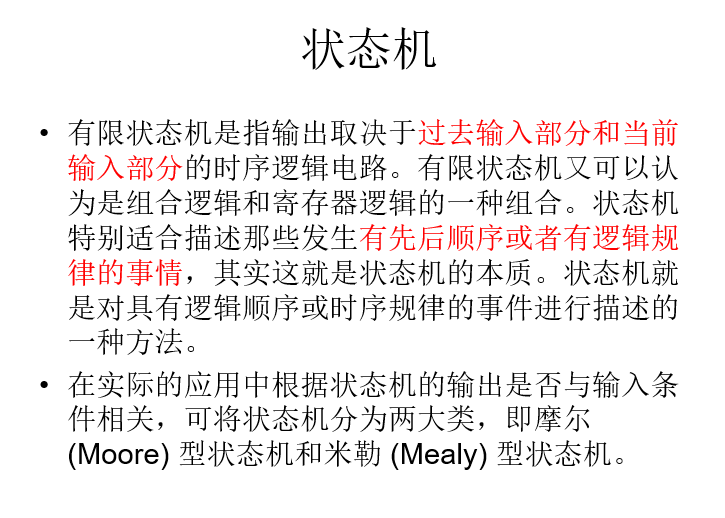
\includegraphics[width=1\textwidth]{fsm.png}
\end{figure}


\section{实验要求}
\subsection{总体要求}
\paragraph{1}使用状态机控制运算过程(数据读取,计算,数据写入),每部加法运算所用时钟数不允许超过五个。典型的,三个clk读取数据和操作符,一个clk计算,一个clk向ram写入结果。
\paragraph{2}仿真激励文件模块只允许出现clk和rst信号输入。
\paragraph{3}本次实验参考所用周期数进行评分,周期越多分越低。

\subsection{设计要求}
实现一个control模块,完成整个运算的控制。
实现一个顶层模块Top
调用Ram模块
调用RegFile
调用ALU完成加法运算
调用control模块,完成运算控制

\subsection{功能要求}
\paragraph{1}通过例化,向ram中0地址到13地址存入14个数,比如10-23;向ram中100地址到106地址存入7个数,比如0~6,分别代表运算符(与ALU的操作符对应),最后向ram 107地址写入-1
\paragraph{2}运算控制:
从ram 0地址开始的地方取两个数,分别放在reg0和reg1,然后从ram 100地址开始的地方取一个运算符,放到reg2,计算之后,把结果存入ram地址200
从ram 2地址开始的地方取两个数,分别放在reg0和reg1,从ram 101地址开始的地方取一个运算符,放到reg2,计算之后,把结果存入ram地址201
……
如果取出操作符为-1,则结束。


\section{实验分析}
\paragraph{1}设计顶层模块,及各模块的接口
\paragraph{2}设计fsm用来control, 各状态的动作, 三段式的实现
\paragraph{3}注意到时序同步的, 所以交替使用上升沿和下降沿
\paragraph{4}
初始化,
检查control中的状态, 传给top, 前3个周期读,
此时也是通过control传递en, addr, 等信息,
将得到的输入信息传到control后,用导线?连接到alu,
alu再将计算结果传回control,
由control再写ram


\section{仿真结果}
\begin{figure}[H]
  \centering
  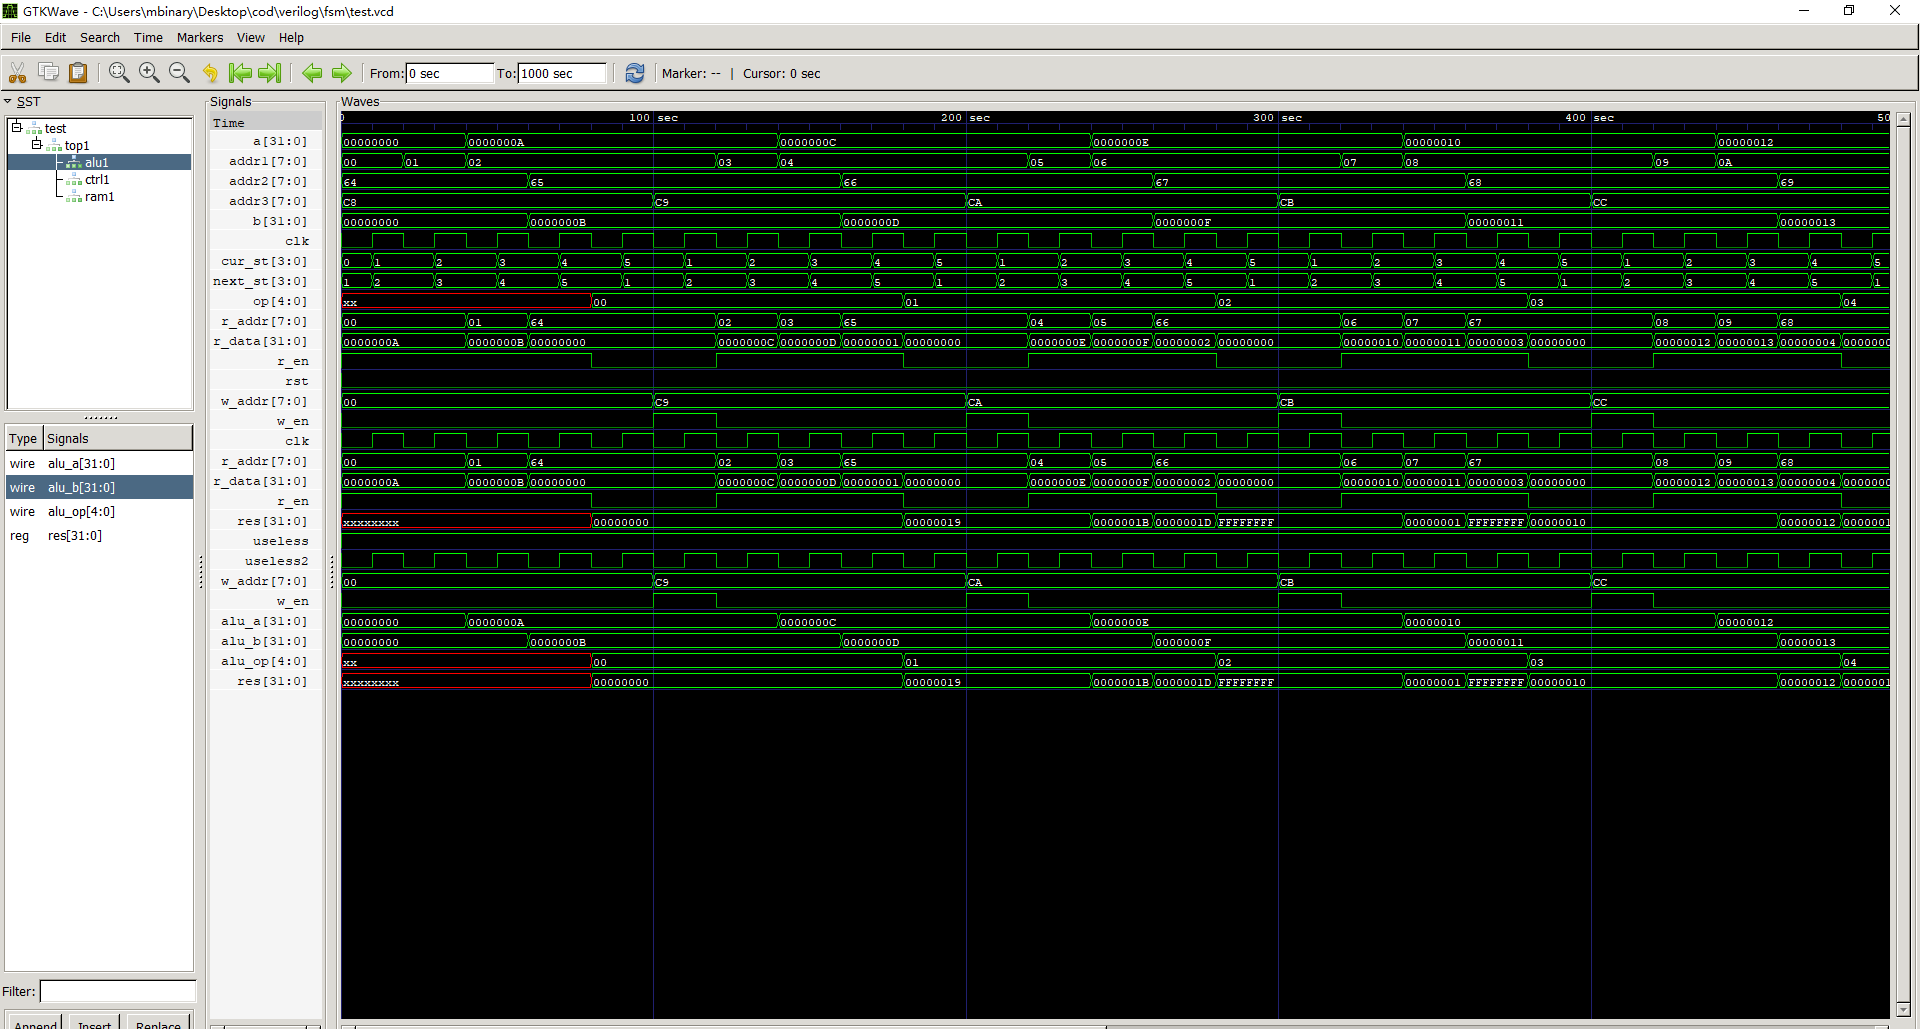
\includegraphics[width=1\textwidth]{wave.png}
\end{figure}



\section{源代码}

\begin{lstlisting}[language=verilog],

//test
module test();
    
reg clk=0,rst=0;

initial begin 
    $dumpfile("test.vcd");
    $dumpvars(0,test);
    #1000 ;
    $finish;
end

top top1(clk,rst);

always #10 
begin 
    clk = ~clk;
end


endmodule



//top
module top(
    input wire clk,
    input wire rst
    );
    
wire w_en,r_en;
wire [7:0] r_addr,w_addr;
wire [31:0] r_data,a,b,res;
wire [4:0] op;
alu alu1(a,b,op,res);
control ctrl1(clk,rst,w_en,w_addr,r_en,r_addr,r_data,a,b,op);
ram ram1(clk,w_en,1,w_addr,res,clk,r_en,r_addr,r_data);
endmodule



//ram
module ram(
    input clk,
    input  w_en,useless,
    input [7:0] w_addr,
    input [31:0]res,
    input useless2,r_en,
    input [7:0] r_addr,
    output reg[31:0] r_data
    );


	reg [31:0] data [0:255];

    
    initial begin
    data[0] = 10;
data[1] = 11;
data[2] = 12;
data[3] = 13;
data[4] = 14;
data[5] = 15;
data[6] = 16;
data[7] = 17;
data[8] = 18;
data[9] = 19;
data[10] = 20;
data[11] = 21;
data[12] = 22;
data[13] = 23;
data[14] = 0;
data[15] = 0;
data[16] = 0;
data[17] = 0;
data[18] = 0;
data[19] = 0;
data[20] = 0;
data[21] = 0;
data[22] = 0;
data[23] = 0;
data[24] = 0;
data[25] = 0;
data[26] = 0;
data[27] = 0;
data[28] = 0;
data[29] = 0;
data[30] = 0;
data[31] = 0;
data[32] = 0;
data[33] = 0;
data[34] = 0;
data[35] = 0;
data[36] = 0;
data[37] = 0;
data[38] = 0;
data[39] = 0;
data[40] = 0;
data[41] = 0;
data[42] = 0;
data[43] = 0;
data[44] = 0;
data[45] = 0;
data[46] = 0;
data[47] = 0;
data[48] = 0;
data[49] = 0;
data[50] = 0;
data[51] = 0;
data[52] = 0;
data[53] = 0;
data[54] = 0;
data[55] = 0;
data[56] = 0;
data[57] = 0;
data[58] = 0;
data[59] = 0;
data[60] = 0;
data[61] = 0;
data[62] = 0;
data[63] = 0;
data[64] = 0;
data[65] = 0;
data[66] = 0;
data[67] = 0;
data[68] = 0;
data[69] = 0;
data[70] = 0;
data[71] = 0;
data[72] = 0;
data[73] = 0;
data[74] = 0;
data[75] = 0;
data[76] = 0;
data[77] = 0;
data[78] = 0;
data[79] = 0;
data[80] = 0;
data[81] = 0;
data[82] = 0;
data[83] = 0;
data[84] = 0;
data[85] = 0;
data[86] = 0;
data[87] = 0;
data[88] = 0;
data[89] = 0;
data[90] = 0;
data[91] = 0;
data[92] = 0;
data[93] = 0;
data[94] = 0;
data[95] = 0;
data[96] = 0;
data[97] = 0;
data[98] = 0;
data[99] = 0;
data[100] = 0;
data[101] = 1;
data[102] = 2;
data[103] = 3;
data[104] = 4;
data[105] = 5;
data[106] = 6;
data[107] = -1;
end
	always@(*)begin
		if(w_en)data[w_addr] = res;
        else data[w_addr]=data[w_addr];
        if(r_en)r_data = data[r_addr];
        else r_data = 0;
    end
endmodule



//alu
module alu(
        input         [31:0] alu_a,
		input         [31:0] alu_b,
		input 		  [4:0] alu_op,
		output 	reg   [31:0] res);

		always@(*)
		begin
			case(alu_op)
			0:res=0;
			1:res=alu_a+alu_b;
			2:res=alu_a-alu_b;
			3:res=alu_a&alu_b;
			4:res=alu_a|alu_b;
			5:res=alu_a ^ alu_b;
			6:res= ~(alu_a|alu_b);

			endcase
		end
endmodule


//control  fsm
module control(
    input clk,rst,
    output reg  w_en,
    output reg [7:0] w_addr,
    output reg r_en,
    output reg [7:0] r_addr,
    input [31:0] r_data,
    output reg [31:0] a,b,
    output reg [4:0]op
    );
    
    /* port */
/* reg w_en,r_en;
reg [5:0] r_addr,w_addr;
reg [31:0] r_data,a,b;
reg [4:0] op; */

/* inner */
reg [7:0] addr1,addr2,addr3;
reg [3:0] cur_st = 0, next_st=0;// 1,2,3,4,5


always@(posedge clk or posedge rst)
begin
    if(rst)
        cur_st = 0;
    else 
        cur_st = next_st;
end

always@(*)
    case(cur_st)
        1:next_st=2;
        2:next_st=3;
        3:next_st=4;
        4:if(r_data==-1) next_st=0; else next_st=5;
        5:next_st=1;
        default:next_st = 1;
    endcase
    
always@(negedge clk or posedge rst)
    if(rst||cur_st==0)begin
        w_en<=0;
        r_en<=1;
        addr1<=0;
        addr2 <= 100;
        addr3<=200;
        r_addr<=0;
        w_addr<=0;
        a<=0;
        b<=0;
    end else if(cur_st==1) begin
        w_en<=0;
        r_en<=1;
        addr1 <= addr1+1;
        r_addr <= addr1;
     end else if (cur_st==2) begin
        w_en<=0;
        r_en<=1;
        addr1 <= addr1+1;
        r_addr <= addr1;
        a<=r_data;
    end else if (cur_st==3) begin
        w_en<=0;
        r_en<=1;
        addr2 <= addr2+1;
        r_addr <= addr2;
        b<=r_data;
    end else if (cur_st==4) begin
        w_en<=0;
        r_en<=0;
        op<=r_data;
    end else if(cur_st==5) begin
        w_en<=1;
        r_en<=0;
        addr3 = addr3+1;
        w_addr <= addr3;
    end
    
endmodule

\end{lstlisting}

\end{document}